% !TeX root = ../main.tex
\chapter{绪论}
\label{chapter:intro}

\section{研究的背景和意义}
\label{intro:sec:background}


数据中心是互联网的 ``大脑'',也是人类存储海量数据、进行大规模计算和提供互联网服务的基础设施。21 世纪第一个十年,数据中心主要处理 Web 网站、搜索引擎等容易并行的任务;通用处理器的高速性能提升也使得专用硬件的优势不甚明显。因此,互联网数据中心多使用大量低成本的标准服务器搭建 \cite{barroso2009datacenter}。

近十年来,大数据与人工智能的兴起改变了数据中心的应用负载特性。一方面,大数据处理、机器学习等负载对算力要求很高。然而,由于摩尔定律的放缓和 Dennard 缩放定律的终结,近十年来,通用处理器的频率提升和多核核数增加都受到功耗墙的限制 \cite{borkar2011future}。因此,通用处理器性能提升 ``免费的午餐'' 已经结束,体系结构的创新迎来了春天,GPU、FPGA、TPU \cite{jouppi2018motivation} 等定制化硬件在数据中心内大量部署。另一方面,大数据处理、机器学习等负载需要多个节点紧密协同处理,对节点间的通信带宽和延迟要求较高。为了给分布式系统高效地提供消息传递和共享内存两种进程间通信范式,在网络方面需要实现高效的消息传递,在存储层面需要实现高性能的共享数据结构存储。因此,近十年来,数据中心网络从 1 Gbps 发展到 40 Gbps,并有向 100 Gbps 演进的趋势。定制化硬件之间的专用互连也成为趋势。如英伟达 CEO 黄仁勋所说,未来的数据中心会像超级计算机一样 \cite{nvidia-datacenter}。

%与此同时,数据中心的运营模式也在经历一场云化的变革。数据中心的算力逐渐集中到少数几家云厂商,每家拥有数以百万计的服务器。由于云数据中心的规模大,云服务商一方面有足够的规模来平摊服务器、板卡甚至芯片的设计和流片成本,另一方面通过软件优化也可以提高性能指标、降低成本,获得可观的经济效益。由于上述应用负载特性的转变和数据中心的云化,工程师获得了从硬件、系统软件到应用程序的全栈优化机会。

与此同时,数据中心的运营模式也在逐步云化,即少数几家云厂商维护数据中心的基础架构,IT 企业只需按需从云厂商租用计算、网络、存储等资源。在云数据中心中,不同的租户(tenant)共享一个巨大的计算、存储和网络资源池。为了实现资源共享和性能隔离,数据中心需要虚拟化的计算、存储和网络。如图 \ref{intro:fig:virt-architecture} 所示,在基础设施作为服务(IaaS)的云服务模式下,计算节点上需要提供虚拟网络、虚拟云存储、虚拟本地存储等服务,实际的网络和云存储资源则位于独立的网络节点和存储节点上。计算节点上的虚拟网络和存储服务把数据中心内物理上分散的网络和存储资源虚拟化成逻辑上统一调配的资源(``多虚一''),如同一台规模巨大的计算机 \cite{barroso2018datacenter}。网络和存储节点则不仅需要把物理资源共享给多个计算节点上不同租户的虚拟机使用(``一虚多''),还需要提供数据处理功能和高层抽象。例如,网络节点需要提供防火墙、负载均衡、加密隧道网关、网络地址转换(NAT)等\textit{网络功能}(Network Function)\footnote{本文中\textit{网络功能}是一个专有名词,并不是指交换机和路由器等网络设备,而是指防火墙等网络基础架构中的功能。};存储节点需要进行数据结构处理以提供对象存储、文件系统存储等高层抽象,还需要进行复制(replication)以实现容灾;除了持久化存储,数据中心还需要提供内存数据结构存储,以支持分布式系统的通信 \footnote{分布式系统的通信有消息传递和共享内存两种范式。消息传递可以直接映射到网络通信。共享内存范式对开发者更友好,可以支持高可用性和可扩放性,在网络互连的分布式系统中需要通过消息传递来实现。然而,共享内存的抽象层次较低,因此大多数分布式系统使用共享数据结构存储来取代共享内存。}。
%第 \ref{chapter:background} 章将详细介绍数据中心虚拟化的背景知识。


\begin{figure}[htbp]
	\centering
	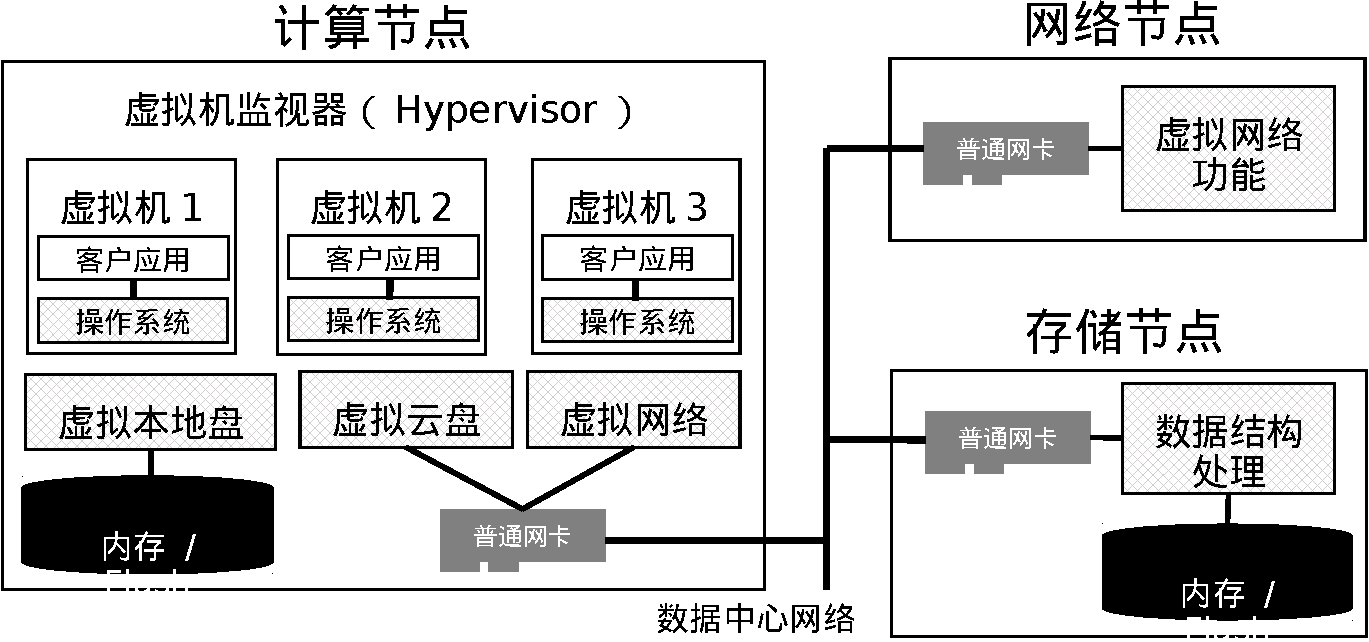
\includegraphics[width=0.8\textwidth]{figures/virt_arch.pdf}
	\caption{虚拟化的数据中心架构。}
	\label{intro:fig:virt-architecture}
\end{figure}


由于云服务的快速迭代,这些虚拟化的网络、存储功能还需要灵活性、可编程性和可调试性,传统上往往用运行在通用处理器上的软件实现。除了虚拟化开销,传统操作系统的开销也不容忽视。这些图 \ref{intro:fig:virt-architecture} 中蓝色方框所示的软件开销被称为 ``数据中心税''(data center tax) \cite{barroso2009datacenter,barroso2013datacenter,barroso2018datacenter}。
在 1 Gbps 网络和机械硬盘的时代,网络、存储虚拟化以及操作系统网络、存储协议栈引入的 CPU 开销和延迟是可以接受的。
在网络、存储、定制化计算硬件越来越快的趋势下,数据中心税不仅浪费了可观的 CPU 资源,还导致应用程序无法充分利用硬件的低延迟和高吞吐量 \cite{barroso2017attack}。
例如,本文第 \ref{chapter:clicknp} 章将说明,计算节点需要分配一部分 CPU 核专门用来实现网络和存储虚拟化,这部分核将无法出售给客户。
此外,虚拟网络和网络功能都会增加数十乃至上千微秒的延迟。作为比较,数据中心网络本身的延迟只有数微秒至数十微秒,虚拟化增加的延迟比网络本身的延迟还高。
第 \ref{chapter:kvdirect} 章将说明,软件实现的内存共享数据结构存储与内存硬件的吞吐量相去甚远。
%如果考虑到存储的数据需要压缩和加密,每个 CPU 核只能处理 100 MB/s 量级的吞吐量,只是一块数据中心级 NVMe SSD 最高吞吐量的约 1/50。
第 \ref{chapter:socksdirect} 章将说明,应用程序普遍使用操作系统中的套接字(socket)原语来进行通信,对于 Web 服务器等通信密集型的应用程序,操作系统占用了很大部分的 CPU 时间;而且,操作系统实现的套接字原语比硬件提供的远程直接内存访问(RDMA)原语延迟高一个数量级。

综上,通过软硬件结合的全栈优化降低 ``数据中心税'' 对现代数据中心的性能和成本有重要意义,这也是本文研究的课题。





\section{国内外研究现状}

为了降低 ``数据中心税'' 的开销,学术界和工业界提出了很多方案,大致可以分为优化软件、利用新型商用硬件和设计新硬件三类。

\subsection{优化软件}

传统的网络功能由部署在数据中心特定位置的专用设备实现。这些专用网络功能设备不仅价格高昂,也不够灵活,不足以支持云服务中的多租户。
为此,云服务商部署了软件实现的虚拟网络功能。例如,Ananta \cite {ananta} 是一个部署在微软数据中心的软件负载均衡器,用于提供云规模的负载均衡服务。
RouteBricks \cite {routebricks} 等工作表明,基于多核 x86 CPU 的每台服务器转发数据包的速度可达 10 Gbps,并且可以通过多核和搭建更多网络节点的集群来扩展容量。
虽然软件实现的虚拟交换机和网络功能可以使用更多数量的 CPU 核和更大的网络节点集群来支持更高的性能,但这样做会增加相当大的资产和运营成本 \cite {ananta,duet}。
云服务商在 IaaS 业务中的盈利能力是客户为虚拟机支付的价格与托管虚拟机的成本之间的差异。
由于每台服务器的资产和运营成本在上架部署时就已基本确定,因此降低托管虚拟机成本的最佳方法是在每台计算节点服务器上打包更多的客户虚拟机,并减少网络和存储节点的服务器数量。
目前,物理 CPU 核(2 个超线程,即 2 个 vCPU)的售价为 0.1 美元/小时左右,亦即最大潜在收入约为 900 美元/年 \cite{smartnic}。
在数据中心,服务器通常服役 3 到 5 年,因此一个物理 CPU 核在服务器生命周期内的售价最高可达 4500 美元 \cite{smartnic}。
即使考虑到总有一部分 CPU 核没有被售出,并且云经常为大客户提供折扣,与专用硬件相比,即使专门分配一个物理 CPU 核用于虚拟网络也是相当昂贵的。

绝大多数应用程序通过操作系统提供的套接字(socket)接口访问网络。Linux 等现有操作系统的套接字是为几十年前的低速网络设计的,在当今高吞吐量、低延迟的数据中心网络中有很高的开销。
近年来,大量工作致力于提供高性能套接字。
第一类工作是优化操作系统内核的 TCP/IP 网络协议栈。
但是,大量的内核开销仍然存在,这将在第 \ref {chapter:socksdirect} 章详细讨论。
第二类工作完全绕过内核 TCP/IP 协议栈并在用户空间中实现 TCP/IP,称为用户态协议栈。
在这个类别中,一些工作 \cite {belay2017ix,peter2016arrakis} 提出了新的操作系统架构,使用虚拟化来确保安全性和隔离性。
除了这些新的操作系统体系结构,许多用户态协议栈利用 Linux 上已经存在的高性能数据包 I/O 框架 \cite {rizzo2012netmap,dpdk,pf-ring}。
其中,一些用户态协议栈 \cite {marinos2014network,jeong2014mtcp,seastar,fstack} 认为 Linux 套接字 API 是性能开销的根源,进而提出了新的 API,因此需要修改应用程序。
大多数 API 更改旨在支持零拷贝(zero copy)。
另一些系统  \cite {kalia2016fasst,kalia2018datacenter} 更进一步,认为套接字的抽象层次太低,应用程序应当使用更高层次的远程过程调用(RPC)接口。
由于套接字的应用非常广泛,要求应用程序修改接口在很多情况下并不现实。
因此,工业界 \cite{libvma,openonload,dbl} 和学术界 \cite{huang2017high} 的一些系统提出了符合标准套接字 API 的用户态 TCP/IP 协议栈。
这些用户态协议栈提供了比 Linux 更好的性能,但它仍然不接近硬件的性能极限。
目前,数据中心网络内主机间通信的性能标杆是远程直接内存访问(RDMA),而主机内进程间通信最高效的方法是共享内存(shared memory)。
这些用户态协议栈的主机间通信延迟比 RDMA 高一个数量级,主机内通信延迟比共享内存高一到两个数量级。

作为分布式系统通信和存储的重要基础设施,键值存储(Key-Value Storage)系统的研究和开发一直是系统学术界和工业界的热点。
早期的内存键值存储系统 \cite{memcached} 性能不令人满意。
由于分布式系统是通过网络互连的,键值存储系统的用户客户端和存储服务器之间也需要通过网络通信,引入了前面讨论的套接字网络协议栈和网络虚拟化等开销。
为了摆脱操作系统内核的开销,近期的键值存储系统  \cite {kapoor2012chronos,ousterhout2010case,ousterhout2015ramcloud,lim2014mica,li2016full} 利用高性能网络数据包处理框架,轮询来自网卡的网络数据包,并且使用上文所述的用户态轻量级网络协议栈处理它们。
然而,即使不考虑网络的开销,键值存储系统进行数据结构处理的成本也很高。
为了降低计算成本,一系列工作 \cite{mao2012cache,fan2013memc3,li2014algorithmic} 优化锁、缓存、哈希和内存分配算法。为了降低多个 CPU 核共同处理同一个键的核间同步开销,较高效的办法是由固定的 CPU 核处理每个键的写操作 \cite{lim2014mica}。
然而,由于 CPU 并行性的限制,第 \ref{chapter:kvdirect} 章将讨论,即使优化到极致,每个 CPU 核每秒也只能处理约 500 万次键值操作请求,远低于内存随机访存所能提供的硬件性能。
此外,现实世界工作负载的键往往服从长尾分布,即少量键访问非常频繁,大多数键访问不频繁。在长尾分布负载下,由于同一个键总是映射到同一个 CPU 核,将导致 CPU 核之间的负载不平衡 \cite{lim2014mica}。





\subsection{利用新型商用硬件}


由于大规模 Web 服务、大数据处理、机器学习等应用对计算和网络的性能需求非常迫切,图形处理器(GPU)等计算加速设备和远程直接内存访问(RDMA) \cite{infiniband2000infiniband} 等网络加速技术在越来越多的数据中心广泛部署。

为了加速虚拟网络和网络功能,以前的工作已经提出使用 GPU \cite {packetshader},网络处理器(Network Processor,NP) \cite {cavium,netronome} 和硬件网络交换机 \footnote{本文中,\textit{交换机}(switch)与路由器不加区分,数据中心的相关文献中通常使用\textit{交换机}一词指代网络互连设备。} \cite {duet}。
GPU 早期主要用于图形处理,近年来扩展到具有海量数据并行性的其他应用程序。
PacketShader \cite {packetshader} 表明使用 GPU 可以实现 40Gbps 的分组交换速度。
GPU 适合批量操作,但是,批量操作会导致高延迟。
网络处理器的历史则可以追溯到 20 世纪 90 年代的网络交换机。
网络处理器由大量的嵌入式处理器核心构成,每个处理器核心的处理能力有限,而有状态连接通常由固定的处理器核心处理,从而单条连接的吞吐量有一定的局限性。
硬件网络交换机的主要问题是灵活性和查找表容量不足 \cite {duet}。

为了降低操作系统通信原语的开销,一系列工作将套接字系统的一部分卸载到网卡硬件上。
TCP 卸载引擎(TCP Offload Engine,TOE) \cite {tcp-chimney-offload} 将部分或全部的 TCP / IP 协议栈卸载到网卡,但由于通用处理器的性能按摩尔定律迅速增长,这些专用硬件的性能优势有限,仅在专用领域中获得成功。
近年来,由于数据中心的硬件趋势和应用需求,\emph {有状态}卸载的故事开始复兴 \cite {chuanxiong-rdma-keynote}。
因此,远程直接内存访问(RDMA) \cite {infiniband2000infiniband} 在生产数据中心中广泛使用 \cite {guo2016rdma}。
与基于软件的 TCP / IP 网络协议栈相比,RDMA 使用硬件卸载来提供超低延迟和接近零的 CPU 开销。
为了使套接字应用程序能够使用 RDMA,RSocket 等工作 \cite {rsockets,socketsdirect,russell2008extended} 将套接字操作转换为 RDMA 原语。
它们具有相似的设计,其中 RSocket 的开发最活跃,是套接字转换 RDMA 的事实标准。
但是,RSocket 的性能和兼容性都不令人满意。
第 \ref{chapter:socksdirect} 章将提出一个与现有应用兼容,并能充分利用 RDMA 网卡性能的套接字系统。


为了加速键值存储系统,近年来的工作 \cite {kalia2014using,kalia2016design,kalia2014using,kalia2016design} 利用 RDMA 网卡基于硬件的网络协议栈,使用双面RDMA作为KVS客户端和服务器之间的RPC机制进一步提高每核吞吐量并减少延迟,如图 \ref{intro:fig:memaccess-a} 所示。尽管这些工作进一步降低了网络通信的开销,但如上一节所讨论的,这些系统仍然受到 CPU 的并行性限制。


\begin{figure*}[t]
	\centering
	\subfloat[软件 / 双面 RDMA。\label{intro:fig:memaccess-a}]
	{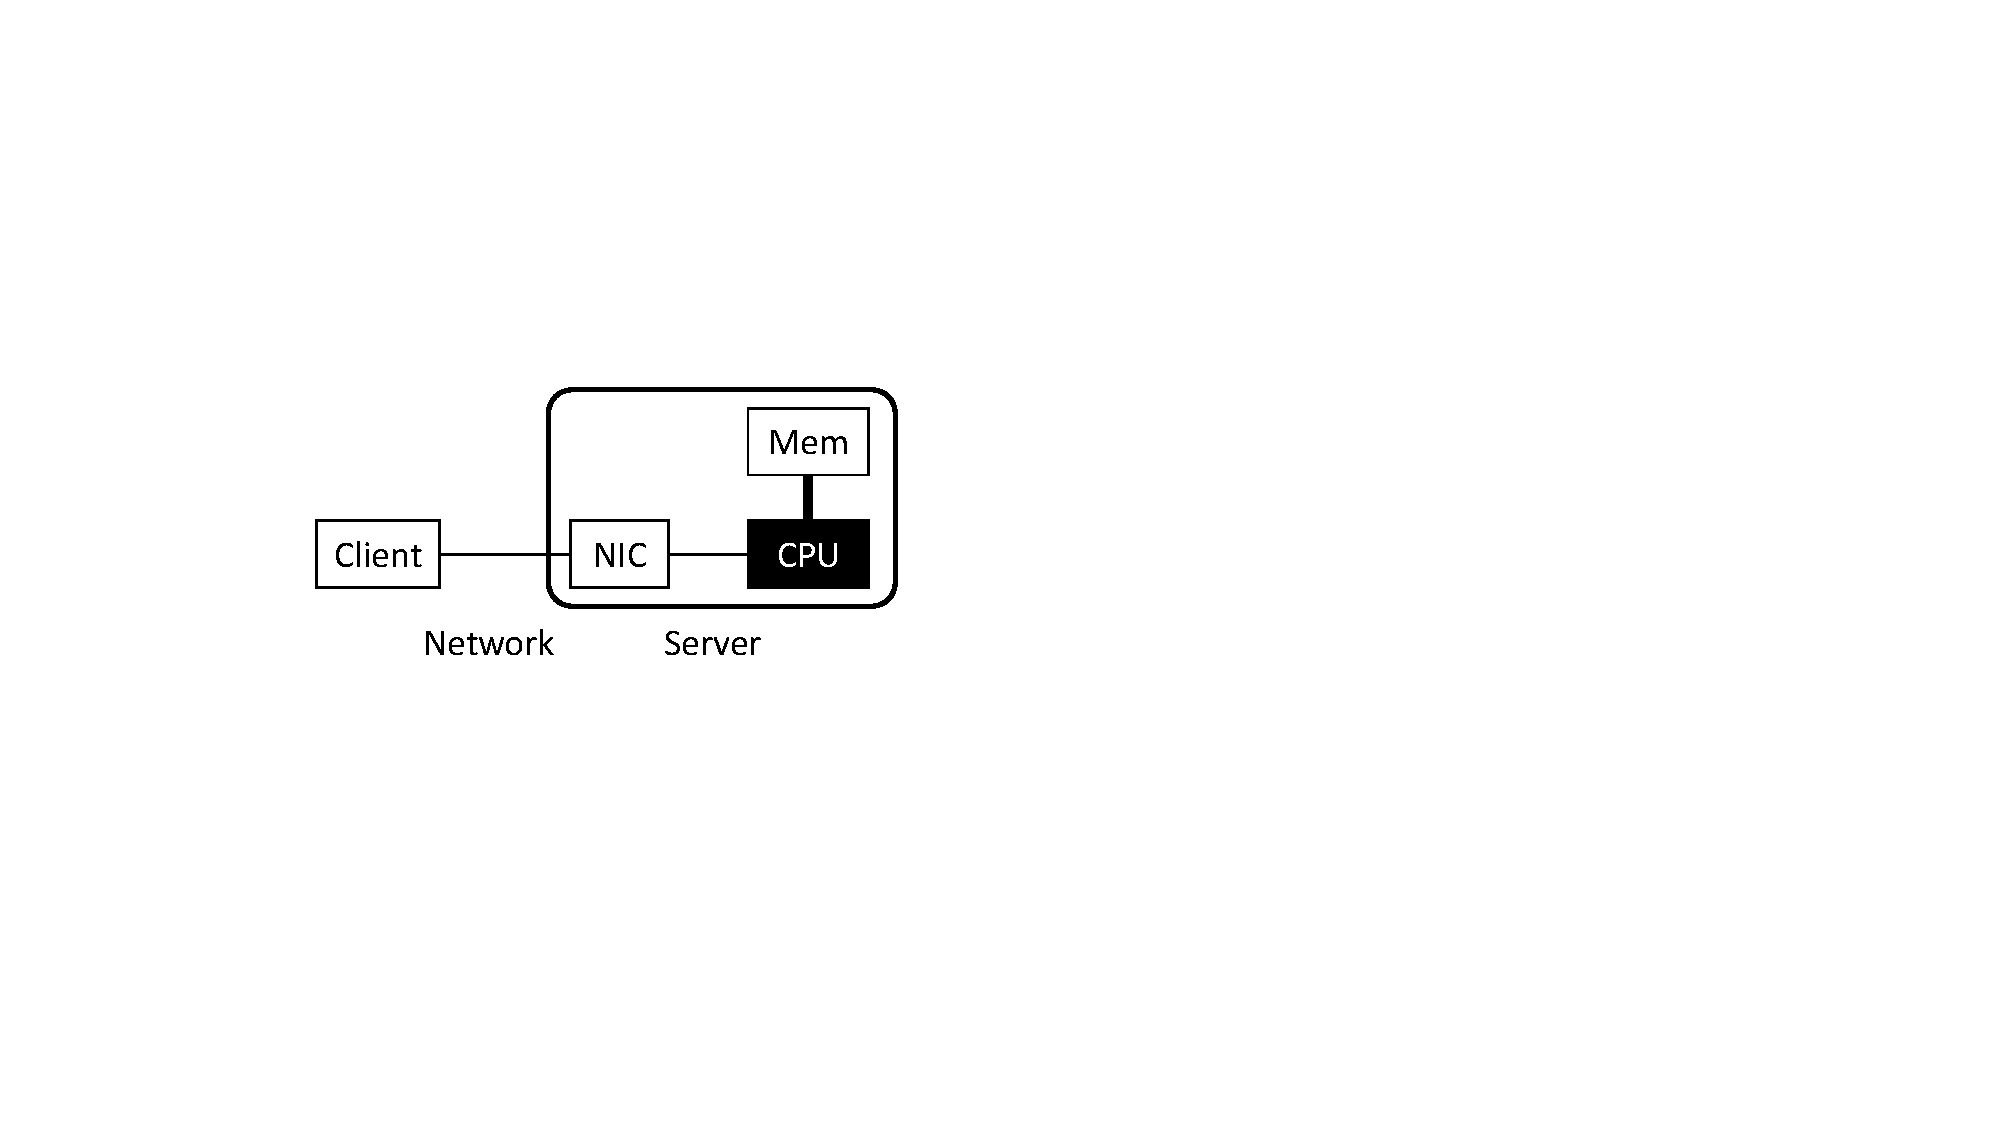
\includegraphics[width=.4\textwidth,page=1]{cropped_access.pdf}}
	\subfloat[单侧 RDMA。\label{intro:fig:kvdirect-b}]
	{\includegraphics[width=.4\textwidth,page=2]{cropped_access.pdf}}
	\caption{键值存储系统的架构。线表示数据路径。一个键值操作(细线)可能需要多个基于地址的存储器访问(粗线)。黑色背景的方框表示键值数据结构处理发生的位置。}
	\label{intro:fig:kvdirect}
\end{figure*}

另一种不同的方法是利用单侧RDMA,如图 \ref{intro:fig:kvdirect-b} 所示。 Pilaf~ \cite {mitchell2013using} 和FaRM~ \cite {dragojevic2014farm} 采用单向RDMA读取进行GET操作,FaRM实现了使网络饱和的吞吐量。 Nessie~ \cite {szepesi2014designing},DrTM~ \cite {wei2015fast},DrTM + R~ \cite {chen2016fast} 和FaSST~ \cite {kalia2016fasst} 利用分布式事务来实现单向RDMA的GET和PUT。但是,PUT操作的性能受到一致性保证的不可避免的同步开销的影响,受到RDMA原语的限制 \cite {kalia2016design}。此外,客户端CPU涉及KV处理,将每个核心的吞吐量限制在客户端的大约10~Mops。
相比之下,本文将RDMA原语扩展到键值操作,同时保证服务器端的一致性,使KVS客户端完全透明,同时实现高吞吐量和低延迟,即使对于PUT操作也是如此。

利用支持 P4 \cite{bosshart2014p4} 的可编程交换机 \cite{barefoot-tofino} 来加速键值存储系统也是近年来研究的热点。
SwitchKV~\cite {li2016fast} 利用基于内容的路由将请求路由到基于缓存键的后端节点,NetCache~ \cite {netcache-sosp17} 进一步将访问频繁的键值缓存在交换机中。
NetChain~\cite{jin2018netchain} 在网络交换机中实现了一个高一致性、容错的键值存储。

为了在键值存储系统中支持事务(transaction),近年来学术界有数据中心网络与共识协议(consensus protocol)共同设计的趋势。
传输顺序在共识协议中至关重要,因此近年来的快速 Paxos~\cite{lamport2006fast,kemme1999processing,moraru2013there,pedone1998optimistic} 协议采用尽力而为的方法提高传输的有序性。
进一步的工作是在网络中提供先入先出(FIFO)和全序(total ordering)的传输顺序保证。
Speculative Paxos~\cite{ports2015designing} 和 NOPaxos~\cite{li2016just} 利用可编程交换机作为中心化的序列号发生器或序列化点。
NetPaxos \cite{dang2015netpaxos,dang2016paxos} 和 \cite{dang2016network} 把传统 Paxos 协议放在网络交换机中实现。
Eris~\cite{eris} 提出使用网络交换机作为序列号发生器,在网络中实现并发控制,实现了快速事务处理。
Hyperloop~\cite{kim2018hyperloop} 在存储节点上利用可编程网卡把写操作写入非易失性内存中的缓冲区,并立即向计算节点回复确认消息,再由存储节点上的软件异步处理非易失性内存中的写操作。这消除了写操作等待存储节点软件处理的延迟。
Google Spanner~\cite{corbett2013spanner} 利用全球同步的 GPS 时钟实现了跨地理区域复制的高性能数据库。



\subsection{设计新硬件}

随着通用处理器的性能提升遇到了瓶颈,各大云服务商开始探索使用定制化硬件来降低 ``数据中心税'',也就是把数据中心的虚拟化、操作系统和高层抽象的开销从通用处理器转移到定制化硬件上。
使用定制化硬件并不是在硬件中原样实现已有的软件,而是对已有软件进行重构,划分出数据面和控制面,数据面优化后在硬件中实现,控制面则留在软件上。
采用新硬件的方案尽管性能较高,但不仅需要新硬件的资产和运营成本,还需要软硬件协同设计的开发成本,往往比单纯优化软件的一次性研发(Non-Recurring Engineering,NRE)成本更高。
此外,相比开发和测试软件,设计、验证和量产新硬件需要较长的研发周期。可编程硬件尽管具有一定的灵活性,但相对通用处理器是受限的,因此需要对未来的数据中心应用负载和基础架构有一定的预见性。
因此,不是所有软件都适合用硬件来加速,需要权衡成本、收益、研发周期、灵活性等多方面的因素。
由于云服务的规模巨大,``数据中心税'' 的开销也很广泛和显著,因此值得设计可编程硬件来加速。

为了尽可能减少计算节点上用于虚拟网络的 CPU 核,以微软 Azure 云为代表的云服务商在数据中心的每台服务器上部署了一块可编程网卡,用以加速虚拟网络 \cite{smartnic}。
为了在提供高性能的同时保持一定的可编程性和灵活性,业界提出了专用芯片(ASIC)、网络处理器(Network Processor)、多核通用处理器片上系统(SoC)、现场可编程门阵列(FPGA)等可编程网卡架构,将在 \ref{smartnic-architecture} 节中详细讨论。
学术界也提出了多种可编程网卡架构。
例如,FlexNIC \cite{kaufmann2016high} 提供了调度、卸载和包分类等新网卡功能。
基于专用芯片的柜顶交换机和可编程网卡灵活性较差,而基于通用处理器的可编程网卡和 GPU 有一定的性能局限性。
FPGA 在性能和灵活性间达到了折中,因此微软采用了基于 FPGA 的可编程网卡 \cite{putnam2014reconfigurable},将在第 \ref{chapter:background} 章中详细介绍。

一些早期的工作已探索在 FPGA 上构建键值存储系统。但是其中一些只使用片上数据存储(大约几MB内存) \cite {liang16fpl} 或板载 DRAM(例如8 GB内存) \cite {istvan2013flexible,chalamalasetti2013fpga,istvan2015hash},因此存储容量有限。
工作 \cite {blott2015scaling} 专注于提高系统容量而不是吞吐量,并采用 SSD 作为板载 DRAM 的二级存储。
工作 \cite {liang16fpl,chalamalasetti2013fpga} 只能存储固定大小的键值对,这样的键值存储系统只能用于一些特定的应用,不够通用。
工作 \cite {blott13hotcloud,lavasani2014fpga} 使用主机 DRAM 存储哈希表,而工作 \cite {tokusashi2016multilevel} 使用网卡 DRAM 作为主机 DRAM 的缓存,但它们没有针对网络和 PCIe DMA 带宽进行优化,导致性能不佳。
本文第 \ref{chapter:kvdirect} 章充分利用了网卡 DRAM 和主机 DRAM,使基于FPGA的键值存储系统通用,并且能够进行大规模部署。此外,精心的软硬件协同设计,以及对PCIe和网络的优化,将性能推向了硬件极限。



FPGA 长期被用于实现网络路由器和交换机。
NetFPGA \cite{lockwood2007netfpga} 提出了一个在 FPGA 上实现路由器的开放硬件平台。
近年来,FPGA 也被用于加速网络功能 \cite {rubow2010chimpp,lavasani2012compiling}。
早在 Click 模块化路由器 \cite{kohler2000click} 编程框架被提出的第二年,Xilinx 就提出了用 FPGA 实现 Click 的 Cliff \cite{kulkarni2004mapping},需要硬件开发人员使用硬件描述语言把一个 Click 元件实现为一个硬件模块。
此后,CUSP \cite{schelle2005cusp} 和 Chimpp \cite {rubow2010chimpp} 提出了一系列改进,简化了硬件模块的互连,提高了软硬件协同处理、软件仿真的能力。
然而,上述工作使用 Verilog、VHDL 等硬件描述语言编程 FPGA。众所周知,硬件描述语言难以调试、编写和修改,给软件人员使用 FPGA 带来了很大挑战。

为了提高 FPGA 的开发效率,FPGA厂商提供了高层次综合(HLS)工具~\cite{vivado,intel-hls},可以把受限的 C 代码编译成硬件模块。学术界和工业界提出了 Bluespec \cite{bluespec}、Lime \cite{auerbach2010lime} 和 Chisel \cite{bachrach2012chisel} 等高效硬件开发语言 \cite{bacon2013fpga,singh2011implementing,wester2015transformation},但它们需要开发者具有足够的硬件设计知识。Gorilla \cite {lavasani2012compiling} 为 FPGA 上的数据包交换提出了一种领域特定的高级语言。但这些工具只是硬件开发工具链的补充,程序员仍然需要手动将从C语言生成的硬件模块插入到硬件描述语言的项目中,且 FPGA 与主机 CPU 之间的通信也需要自行处理。高层次综合工具和高效硬件开发语言可以提高硬件开发人员的工作效率,但仍然不足以让软件开发人员使用 FPGA。

近年来,为了让软件开发人员使用FPGA,FPGA厂商提出了基于OpenCL的编程工具链~\cite{aoc,sdaccel},提供了类似GPU的编程模型,如图 \ref{intro:fig:opencl} 所示。软件开发人员可以把用OpenCL语言编写的核(kernel)卸载到FPGA上。但是,这种方法中多个并行执行的核间需要通过板上共享内存进行通信,而FPGA上的DRAM共享内存吞吐量和延迟都不理想,共享内存还会成为通信瓶颈。其次,FPGA与CPU之间的通信模型是类似GPU的批处理模型,这使得处理延迟较高(约1毫秒),不适用于需要微秒级延迟的网络数据包处理。


\begin{figure}[htbp]
	\centering
	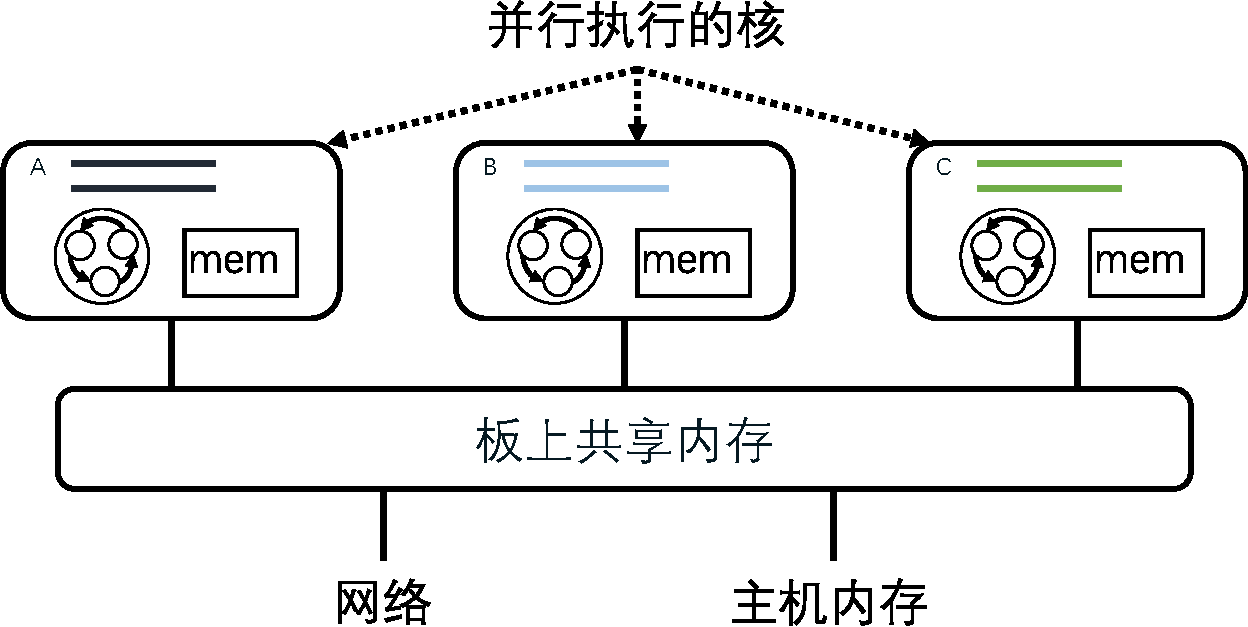
\includegraphics[width=0.7\textwidth]{figures/opencl.pdf}
	\caption{基于 OpenCL 的 FPGA 编程工具链。}
	\label{intro:fig:opencl}
\end{figure}


Click2NetFPGA~\cite {Click2NetFPGA} 利用高层次综合工具,直接将 Click 模块化路由器 \cite {kohler2000click} 的 C++ 代码编译到 FPGA 来提供模块化架构。
然而,Click2NetFPGA 的性能的系统设计存在若干瓶颈(例如,内存和数据包 I/O),它们也没有优化代码以确保完全流水线处理,因此比本文达到的性能低两个数量级。
此外,Click2NetFPGA 不支持 FPGA / CPU 联合处理,因此无法在数据平面运行时更新配置或读取状态。

本文第 \ref{chapter:clicknp} 章将提出一个让软件开发人员可用,且网络数据包处理性能高的模块化 FPGA 编程框架。









\section{本文的研究内容和贡献}


本文旨在探索基于可编程网卡的高性能数据中心系统。本文提出一个基于 FPGA 可编程网卡,对云计算数据中心计算、网络、存储节点实现全栈加速的系统。如图 \ref{intro:fig:accel-arch} 所示,通过把计算、网络、存储节点上的普通网卡替换为可编程网卡,本文在计算节点上实现了虚拟网卡和虚拟网络,虚拟本地存储和云存储,以及轻量级用户态运行库和硬件传输协议相结合的通信原语,替代了图 \ref{intro:fig:virt-architecture} 中的软件虚拟化服务和操作系统网络协议栈。本文还基于数据面与控制面分离的思想,实现了网络节点的虚拟网络功能和存储节点的数据结构处理,用可编程网卡提高数据面性能,并保留原有软件控制面的灵活性。


\begin{figure}[htbp]
	\centering
	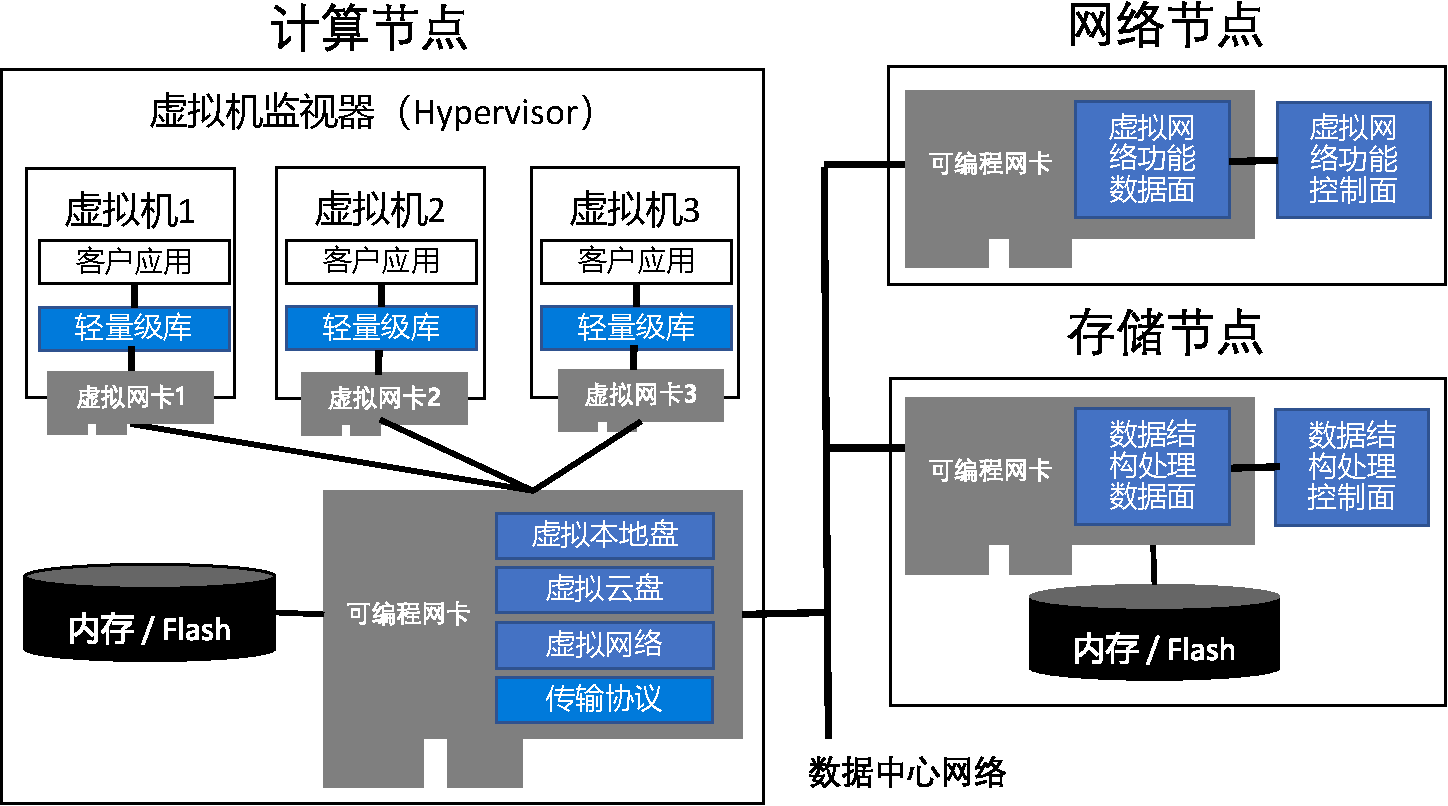
\includegraphics[width=0.8\textwidth]{figures/accel_arch.pdf}
	\caption{基于可编程网卡的数据中心系统总体架构。}
	\label{intro:fig:accel-arch}
\end{figure}

首先,本文提出用可编程网卡加速云计算中的虚拟网络功能。提出了首个在商用服务器中用 FPGA 加速的高灵活性、高性能网络功能处理平台 ClickNP。众所周知,FPGA 编程对软件工程师很不友好。为了简化 FPGA 编程,设计了类 C 的 ClickNP 语言和模块化的编程模型,并开发了一系列优化技术,以充分利用 FPGA 的海量并行性。实现了 ClickNP 开发工具链,可以与多种商用高层次综合工具集成。基于 ClickNP 设计和实现了 200 多个网络元件,并用这些元件组建起多种网络功能。相比基于 CPU 的软件网络功能,ClickNP 的吞吐量提高了 10 倍,延迟降低到 1/10;且具有可忽略的 CPU 开销,可以为云计算中的每个计算节点节约 20\% 的 CPU 核。

其次,本文提出用可编程网卡加速远程数据结构访问。键值存储是最常用的基本数据结构之一,也是很多数据中心内的关键分布式系统组件。基于 ClickNP 编程框架,设计实现了一个高性能内存键值存储系统 KV-Direct,在服务器端绕过 CPU,用可编程网卡通过 PCIe 直接访问主机内存。把单边 RDMA 的内存操作语义扩展到键值操作语义,解决了单边 RDMA 操作数据结构时通信和同步开销高的问题。还利用 FPGA 可重配置的特性,允许用户实现更复杂的数据结构。面对网卡与主机内存之间 PCIe 带宽较低、延迟较高的性能挑战,通过哈希表、内存分配器、乱序执行引擎、负载均衡和缓存、向量操作等一系列性能优化,实现了 10 倍于 CPU 的能耗效率和微秒级的延迟,实现了首个单机性能达到 10 亿次每秒的通用键值存储系统。

最后,本文提出用可编程网卡和用户态运行库相结合的方法为应用程序提供系统原语,从而绕过操作系统内核。套接字是操作系统提供的最常用的通信原语。设计实现了一个用户态套接字系统 SocksDirect,与现有应用程序完全兼容,能实现接近硬件极限的吞吐量和延迟,多核性能具有可扩放性,并在高并发负载下保持高性能。分别使用共享内存和 RDMA 实现主机内和主机间的通信。为了支持高并发连接数,本文基于 KV-Direct 实现了一个 RDMA 可编程网卡。通过消除线程间同步、缓冲区管理、大数据拷贝、进程唤醒等一系列开销,SocksDirect 相比 Linux 提升了 7 至 20 倍吞吐量,降低延迟到 1/17 至 1/35,并将 Web 服务器的 HTTP 延迟降低到 1/5.5。


\section{论文结构安排}

本论文的内容结构安排如下:
第 1 章为绪论。
第 2 章介绍数据中心的发展趋势,指出数据中心软硬件结合优化的需求与机遇,讨论可编程网卡的架构,并调研可编程网卡在数据中心的应用。
第 3 章提出基于可编程网卡的数据中心系统架构。
第 4 章是网络加速部分,提出用可编程网卡加速云计算中的虚拟网络功能。为了简化 FPGA 编程,提出首个适用于高速网络数据包处理、基于高级语言的模块化 FPGA 编程框架 ClickNP。
第 5 章是存储加速部分,提出用可编程网卡加速远程数据结构访问,并设计实现一个高性能内存键值存储系统 KV-Direct。
第 6 章是操作系统加速部分,提出用可编程网卡和用户态运行库相结合的方法为应用程序提供操作系统原语,并设计实现一个用户态套接字系统 SocksDirect。
第 7 章总结全文并展望未来研究方向。